\documentclass[10pt,aspectratio=169]{beamer}

\usetheme{AICL}

\usepackage{amsmath, amssymb}
\usepackage{booktabs}
\usepackage{graphicx}
\usepackage{tikz}
\usetikzlibrary{arrows.meta, positioning, shapes.geometric, calc}

\graphicspath{{../Git_code/cellfree-pilot-hybrids/presentation/}{../Git_code/cellfree-pilot-hybrids/figures/}{../figures/}{.}}

\title{Overhead-Aware Robust Pilot Assignment\\
for Cell-Free Massive MIMO}
\subtitle{Beam-Domain Resource Matching with Weighted Pilot Reuse}
\author{Jeonghoo Maeng \and Myoungjin Oh}
\date{Mobile Communication Systems Term Project}

\newcommand{\taup}{\tau_{\mathrm{p}}}
\newcommand{\tauc}{\tau_{\mathrm{c}}}
\newcommand{\tauactual}{\tau_{\mathrm{p}}^{\mathrm{actual}}}
\newcommand{\taudesign}{\tau_{\mathrm{p}}^{\mathrm{design}}}
\newcommand{\BRM}{Beam Resource Matching}
\newcommand{\BWT}{Beam Weighted Threshold}
\newcommand{\TopN}{AP-Top-$N$}
\newcommand{\waa}{w_{\mathrm{aa}}}
\newcommand{\wai}{w_{\mathrm{ai}}}
\newcommand{\wia}{w_{\mathrm{ia}}}

\newenvironment{tightitemize}{%
    \begin{itemize}
        \setlength{\itemsep}{2pt}
        \setlength{\parskip}{0pt}
        \setlength{\parsep}{0pt}
}{%
    \end{itemize}
}

\newcommand{\callout}[1]{%
    \vspace{0.3em}
    {\footnotesize\itshape #1}
}

\begin{document}

% ----------------------------------------------------------------
% Title
% ----------------------------------------------------------------
\begin{frame}[plain]
    \titlepage
\end{frame}

% ----------------------------------------------------------------
% Introduction
% ----------------------------------------------------------------
\section{Introduction}

\begin{frame}{Cell-Free Massive MIMO}
    \footerref{Gao \emph{et al.}, IEEE TVT 73(1):1453--1467, 2024; Mussbah \emph{et al.}, IEEE Commun.\ Lett.\ 28(9):2176--2180, 2024.}
    \footnotesize
    \begin{columns}[T,onlytextwidth]
        \begin{column}{0.50\textwidth}
            \textbf{System characteristic}
            \begin{tightitemize}
                \item Many distributed APs jointly serve a smaller number of UEs (\(L\gg K\)), coordinated by a central processing unit (CPU) over fronthaul.
                \item No cell boundaries; coherent cooperative transmission yields handover-free coverage.
            \end{tightitemize}
            
            \vspace{0.5em}
            \textbf{Why cell-free mMIMO}
            \begin{tightitemize}
                \item Distributed APs shorten access distances and improve macro-diversity.
                \item Cell-free cooperation reduces cell-edge effects and SINR disparity.
                \item Dense AP--UE connectivity also creates many overlapping spatial links, making pilot reuse a central bottleneck.
            \end{tightitemize}
        \end{column}
        \begin{column}{0.48\textwidth}
            \centering
            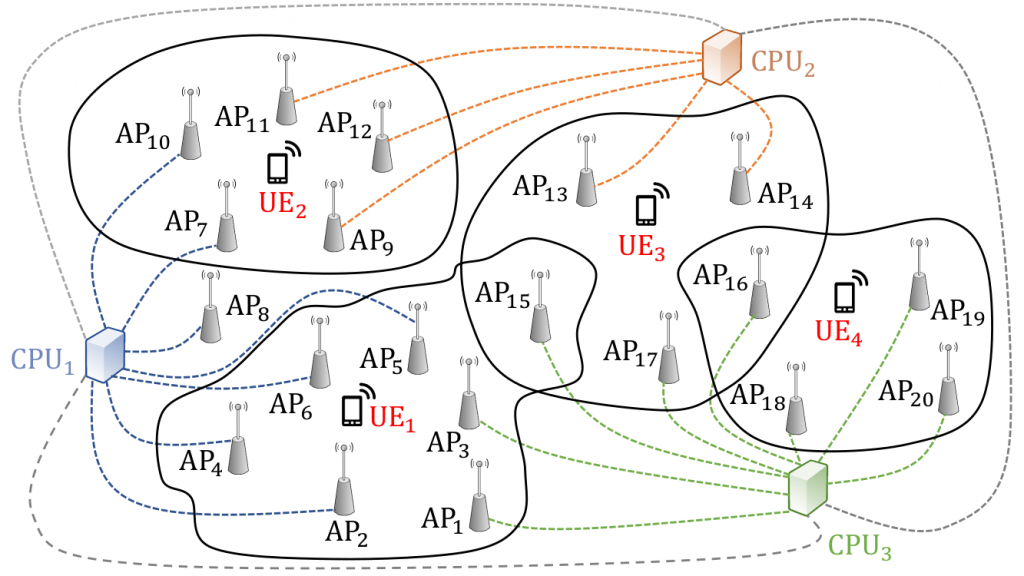
\includegraphics[width=\linewidth,height=0.72\textheight,keepaspectratio]{CF_system.png}
        \end{column}
    \end{columns}
\end{frame}

\begin{frame}{The Pilot Problem}
    \small
    \begin{columns}[T,onlytextwidth]
        \begin{column}{0.50\textwidth}
            \textbf{Channel estimation via uplink pilots}
            
            A TDD coherence block of length \(\tauc\) allocates \(\taup\) pilot symbols followed by \(\tauc-\taup\) data symbols. AP \(l\) receives
            \[
                \mathbf{Y}_{\mathrm{p},l}
                =
                \sum_{k=1}^{K}
                \sqrt{\taup\rho_{\mathrm{p}}}\,
                \mathbf{h}_{k,l}\boldsymbol{\phi}_{p_k}^{H}
                +
                \mathbf{N}_{\mathrm{p},l},
            \]
            where \(p_k\) is the pilot index assigned to UE \(k\). Correlating with \(\boldsymbol{\phi}_{p_k}\) gives the observation used for MMSE channel estimation.
            
            \vspace{0.4em}
            \[
                \mathrm{SE}_k = \frac{\tauc - \taup}{\tauc}\,\log_2(1+\mathrm{SINR}_k).
            \]
        \end{column}
        \begin{column}{0.46\textwidth}
            \textbf{Pilot contamination}
            \begin{tightitemize}
                \item Typically \(K>\taup\); UEs must reuse pilots.
                \item Same-pilot UEs corrupt one another's MMSE estimates.
                \item Contamination severity scales with the overlap of serving APs and beam directions among pilot-sharing UEs.
            \end{tightitemize}
            
            \vspace{0.45em}
            \begin{block}{Design goal}
                Assign pilots so that same-pilot UEs share as little spatial structure as possible.
            \end{block}
        \end{column}
    \end{columns}
\end{frame}

\begin{frame}{Prior Approaches and Gap}
    \small
    \begin{columns}[T,onlytextwidth]
        \begin{column}{0.48\textwidth}
            \textbf{Gao (TVT 2024): AP-domain matching}
            \begin{tightitemize}
                \item Group UEs by common serving APs.
                \item Many-to-many matching between UEs and APs.
                \item Orthogonal pilots within high-risk groups.
            \end{tightitemize}
            
            \vspace{0.3em}
            \callout{Limitation: AP-level matching does not resolve beam direction within a shared AP.}
        \end{column}
        \begin{column}{0.48\textwidth}
            \textbf{Mussbah (IEEE CL 2024): Beam-domain graph}
            \begin{tightitemize}
                \item Beam-domain channel decomposition (DFT codebook).
                \item Active / moderate beam reports from initial access.
                \item Pilot assignment by graph coloring on beam overlap.
            \end{tightitemize}
            
            \vspace{0.3em}
            \callout{Limitation: dense beam-overlap graphs inflate the chromatic number and pilot overhead.}
        \end{column}
    \end{columns}
    
    \vspace{0.6em}
    \begin{block}{This work}
        \BRM{} combines Gao's matching mechanism with Mussbah's beam-domain structure: many-to-many matching at the AP-beam resource level \(r=(l,n)\).
    \end{block}
\end{frame}

% ----------------------------------------------------------------
% Core summary
% ----------------------------------------------------------------
\section{Overview}

\begin{frame}{Core Design Concept}
    \small
    \begin{block}{Design principle}
        \BRM{} lifts Gao's many-to-many matching from the AP domain to the AP-beam
        resource domain and inherits Mussbah's active/moderate beam structure.
    \end{block}
    
    \vspace{0.5em}
    \begin{center}
        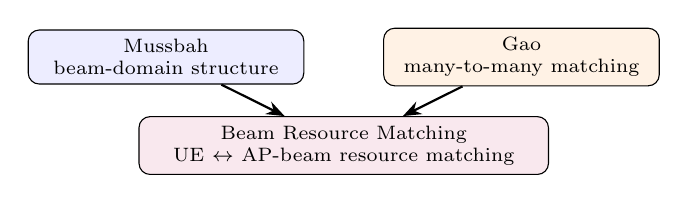
\begin{tikzpicture}[
                node distance=0.55cm,
                box/.style={draw, rounded corners, align=center, minimum width=3.5cm, minimum height=0.62cm, font=\scriptsize, fill=blue!7},
                arr/.style={->, thick, >=Stealth}
            ]
            \node[box] (m) {Mussbah\\beam-domain structure};
            \node[box, right=1.0cm of m, fill=orange!10] (g) {Gao\\many-to-many matching};
            \node[box, below=0.75cm of $(m)!0.5!(g)$, fill=purple!9, minimum width=5.2cm] (b) {\BRM{}\\UE $\leftrightarrow$ AP-beam resource matching};
            \draw[arr] (m) -- (b);
            \draw[arr] (g) -- (b);
        \end{tikzpicture}
    \end{center}
    
    \vspace{0.3em}
    \begin{tightitemize}
        \item \textbf{Gao}: many-to-many matching between UEs and APs on large-scale fading.
        \item \textbf{Mussbah}: beam-domain conflict graph from active/moderate beam overlaps.
        \item \textbf{\BRM{}}: matches UEs to resources \(r=(l,n)\); the matching outcome determines the active beam set and feeds pilot assignment.
    \end{tightitemize}
\end{frame}

% ----------------------------------------------------------------
% Reference methods
% ----------------------------------------------------------------
\section{Reference Methods}

\begin{frame}{Mussbah Beam-Domain Method}
    \footerref{Mussbah \emph{et al.}, IEEE Commun.\ Lett.\ 28(9):2176--2180, 2024.}
    \small
    \begin{columns}[T,onlytextwidth]
        \begin{column}{0.49\textwidth}
            \textbf{Beam-domain channel}
            \[
                \mathbf{h}_{k,l}^{(B)}=\mathbf{U}^{H}\mathbf{h}_{k,l}.
            \]
            UE \(k\) reports beam set \(\mathcal{B}_k\). The strongest beams (cumulative power threshold) form the active set:
            \[
                \mathcal{B}_k^{(a)} \subset \mathcal{B}_k.
            \]
            Remaining reported beams form the moderate set:
            \[
                \mathcal{B}_k^{(i)}
                =
                \mathcal{B}_k\setminus\mathcal{B}_k^{(a)}.
            \]
        \end{column}
        \begin{column}{0.47\textwidth}
            \textbf{Conflict graph}
            \[
                \mathbf{B}
                =
                \mathbf{B}^{(a)T}\mathbf{B}^{(a)}
                +
                \mathbf{B}^{(a)T}\mathbf{B}^{(i)}
                +
                \mathbf{B}^{(i)T}\mathbf{B}^{(a)}.
            \]
            \[
                A_{i,j}=1 \quad \text{if } B_{i,j}>0.
            \]
            Pilots are assigned by graph coloring:
            \[
                \tauactual = \chi(G).
            \]
            
            \vspace{0.25em}
            \textbf{Energy efficiency}
            \[
                \begin{aligned}
                    \mathrm{EE}
                     & =
                    \frac{B_{\mathrm{w}}\sum_{k=1}^{K}\mathrm{SE}_k}{P_{\mathrm{tot}}}, \\
                    P_{\mathrm{tot}}
                     & =
                    P_{\mathrm{tx}}+P_{\mathrm{c}}+N_{\mathrm{RF}}P_{\mathrm{RF}}.
                \end{aligned}
            \]
            \scriptsize Active-beam selection reduces \(N_{\mathrm{RF}}\) through RF-chain on/off.
        \end{column}
    \end{columns}
    
    \begin{tikzpicture}[remember picture,overlay]
        \node[
            anchor=south west,
            align=left,
            text width=0.86\paperwidth
        ] at ([xshift=0.63cm,yshift=0.60cm]current page.south west) {%
            {\scriptsize\itshape
                    Beam-domain conflicts capture finer interference than AP-domain.\\[-0.1em]
                    Trade-off: dense graphs raise the chromatic number and inflate pilot overhead.
                }%
        };
    \end{tikzpicture}
\end{frame}

\begin{frame}{DSATUR coloring (Mussbah)}
    \small
    \begin{block}{Core idea}
        Among uncolored vertices, DSATUR colors first the vertex with the largest saturation degree.
    \end{block}
    
    \vspace{-0.2em}
    \[
        d_{\mathrm{sat}}(v)
        =
        \left|
        \{c_u:\ u\in\mathcal{N}(v),\ c_u\neq -1\}
        \right|.
    \]
    \vspace{-0.7em}
    \[
        d_{\mathrm{sat}}(v)
        =
        \text{number of distinct colors already used by colored neighbors of } v.
    \]
    
    \vspace{0.1em}
    \centering
    \scriptsize
    \begin{tabular}{cll}
        \toprule
        Step & Operation                                & Meaning                                \\
        \midrule
        1    & Initialize \(c_k=-1,\ \forall k\)        & all UEs are uncolored                  \\
        2    & Compute degree \(d(v)=|\mathcal{N}(v)|\) & static conflict count                  \\
        3    & Select uncolored vertex                  & choose largest \(d_{\mathrm{sat}}(v)\) \\
        4    & Tie-breaking                             & if tied, choose largest \(d(v)\)       \\
        5    & Assign color                             & smallest color unused by neighbors     \\
        6    & Update saturation degree                 & update neighbors' \(d_{\mathrm{sat}}\) \\
        7    & Repeat                                   & until every UE receives a color        \\
        \bottomrule
    \end{tabular}
    
    \vspace{0.45em}
    \callout{In Mussbah, vertices are UEs and graph edges come from active/moderate beam overlap. The number of colors becomes the actual pilot count \(\tauactual=\chi(G)\).}
\end{frame}

\begin{frame}{Beam Weighted Threshold}
    \small
    \begin{block}{Design objective}
        \BWT{} retains Mussbah's beam-domain coloring framework while suppressing weak edges through a weighted interference score.
    \end{block}
    
    \vspace{0.4em}
    \[
        B_{u,v}^{w}
        =
        \waa\,|\mathcal{B}_{u}^{(a)}\cap\mathcal{B}_{v}^{(a)}|
        +
        \wai\,|\mathcal{B}_{u}^{(a)}\cap\mathcal{B}_{v}^{(i)}|
        +
        \wia\,|\mathcal{B}_{u}^{(i)}\cap\mathcal{B}_{v}^{(a)}|.
    \]
    
    \[
        A_{u,v}
        =
        \begin{cases}
            1, & B_{u,v}^{w}>\theta,\ u\neq v, \\
            0, & \text{otherwise.}
        \end{cases}
    \]
    
    \vspace{0.3em}
    \begin{tightitemize}
        \item \(\waa\) emphasizes active-active overlap, the typically dominant interference.
        \item Threshold \(\theta\) controls graph density.
        \item Pilots are assigned by graph coloring on \(G_{\theta}\):
        \[
            \tauactual = \chi(G_{\theta}).
        \]
    \end{tightitemize}
\end{frame}

\begin{frame}{Gao AP-Domain Matching}
    \footerref{Gao \emph{et al.}, IEEE Trans.\ Veh.\ Technol.\ 73(1):1453--1457, 2023.}
    \small
    \begin{columns}[T,onlytextwidth]
        \begin{column}{0.50\textwidth}
            Gao performs many-to-many matching between UEs and APs based on AP-domain large-scale fading \(\beta_{m,k}\). The indicator
            \[
                \mu(m,k)=1
            \]
            denotes that UE \(m\) is matched to AP \(k\).
            
            \vspace{0.4em}
            \textbf{Quota constraints}
            \[
                |\mu(\mathrm{UE}_m)| \le Q_{\mathrm{UE}},
                \qquad
                |\mu(\mathrm{AP}_k)| \le Q_{\mathrm{AP}}.
            \]
            Key setting:
            \[
                Q_{\mathrm{AP}}=\taup.
            \]
        \end{column}
        \begin{column}{0.46\textwidth}
            \textbf{AP group}
            \[
                \mathcal{G}_k=\{m:\mu(m,k)=1\}.
            \]
            \textbf{Common serving AP ratio}
            \[
                M_{m_1,m_2}^{AP}
                =
                \frac{|\mu(m_1,:)\cap\mu(m_2,:)|}{|\mu(m_1,:)|}.
            \]
            \textbf{Group risk}
            \[
                S_k
                =
                \sum_{m_1\neq m_2,\ m_1,m_2\in\mathcal{G}_k}
                M_{m_1,m_2}^{AP}.
            \]
        \end{column}
    \end{columns}
    
    \vspace{0.3em}
    \callout{Limitation: AP-level matching cannot distinguish two UEs that share an AP through different beams.}
\end{frame}

\begin{frame}{AP-Top-\(N\) Method}
    \small
    \begin{columns}[T,onlytextwidth]
        \begin{column}{0.50\textwidth}
            \textbf{Sparse AP-domain conflict graph}
            \[
                \mathcal{T}_k(N_{\mathrm{top}})
                =
                \operatorname{Top}_{N_{\mathrm{top}}}
                \{\beta_{k,1},\ldots,\beta_{k,L}\}.
            \]
            A conflict edge is placed when two UEs share at least one Top-\(N\) AP:
            \[
                A_{i,j}
                =
                \mathbf{1}\{
                \mathcal{T}_i(N_{\mathrm{top}})
                \cap
                \mathcal{T}_j(N_{\mathrm{top}})
                \neq \varnothing
                \}.
            \]
        \end{column}
        \begin{column}{0.46\textwidth}
            \textbf{Pilot assignment flow}
            \begin{tightitemize}
                \item Identify the Top-\(N\) strongest APs per UE.
                \item Connect UEs whose Top-\(N\) sets intersect.
                \item Apply graph coloring on the resulting sparse graph.
                \item Connected UEs receive distinct pilots.
            \end{tightitemize}
            
            \vspace{0.6em}
            \begin{block}{Algorithmic role}
                \TopN{} provides a lightweight AP-domain sparsification of Gao's AP-overlap criterion.
            \end{block}
        \end{column}
    \end{columns}
\end{frame}

% ----------------------------------------------------------------
% Beam Resource Matching
% ----------------------------------------------------------------
\section{Beam Resource Matching}

\begin{frame}{Beam Resource Matching (BRM)}
    \small
    \begin{columns}[T,onlytextwidth]
        \begin{column}{0.48\textwidth}
            \textbf{\large Resource definition}
            
            \vspace{0.75em}
            \[
                r=(l,n),
                \qquad
                |\mathcal{R}|=LN.
            \]
            
            \vspace{0.7em}
            {\setbeamertemplate{itemize item}{\color{red!70!black}\scriptsize\(\blacksquare\)}
                \begin{itemize}
                    \setlength{\itemsep}{0.45em}
                    \item \(l\): AP index.
                    \item \(n\): beam index at AP \(l\).
                    \item Each pair \((l,n)\) constitutes a single matching resource.
                \end{itemize}}
            
            \vspace{1.0em}
            \textbf{\large UE-resource preference}
            
            \vspace{0.45em}
            \[
                P_{k,r}=P_{k,l,n}.
            \]
        \end{column}
        \begin{column}{0.49\textwidth}
            \textbf{\large Resolution gain over Gao}
            
            \vspace{0.65em}
            {\setbeamertemplate{itemize item}{\color{red!70!black}\scriptsize\(\blacksquare\)}
                \begin{itemize}
                    \setlength{\itemsep}{0.45em}
                    \item Gao ranks candidates by AP-domain strength \(\beta_{k,l}\).
                    \item Beam Resource Matching ranks by beam-domain power \(P_{k,l,n}\).
                    \item Beam-level resolution separates ``same AP'' from ``same beam.''
                \end{itemize}}
            
            \vspace{1.0em}
            \textbf{\large Modeling distinction}
            
            \vspace{0.55em}
            Matching operates at the AP-beam resource level rather than the AP level.
        \end{column}
    \end{columns}
\end{frame}

\begin{frame}{BRM: Matching Variables and Constraints}
    \small
    \begin{columns}[T,onlytextwidth]
        \begin{column}{0.49\textwidth}
            \textbf{Reference quota}
            \[
                Q_k^{UE}=|\widetilde{\mathcal{A}}_k|.
            \]
            \(\widetilde{\mathcal{A}}_k\) denotes the reference active beam set from the Mussbah power-threshold rule.
            
            \vspace{0.4em}
            \textbf{Matching variable}
            \[
                \mu_{k,r}\in\{0,1\}.
            \]
            \[
                \mu_{k,r}=1
                \quad \Longleftrightarrow \quad
                \text{UE }k\text{ is matched to resource }r.
            \]
        \end{column}
        \begin{column}{0.47\textwidth}
            \textbf{Constraints}
            \[
                \sum_{r\in\mathcal{R}}\mu_{k,r}
                \le Q_k^{UE},
                \qquad
                \sum_{k=1}^{K}\mu_{k,r}
                \le Q_{\mathrm{res}}.
            \]
            \[
                \mu_{k,r}=0
                \quad
                \text{if } r\notin \mathcal{B}_k.
            \]
            Typical choice:
            \[
                Q_{\mathrm{res}}=\taudesign.
            \]
        \end{column}
    \end{columns}
    
    \vspace{0.35em}
    \callout{Matching follows a deferred-acceptance protocol: UEs propose to their strongest resources, and each resource accepts up to \(Q_{\mathrm{res}}\) UEs ranked by beam power.}
\end{frame}

\begin{frame}{Matching Result Defines Active Beams}
    \small
    \begin{columns}[T,onlytextwidth]
        \begin{column}{0.49\textwidth}
            Mussbah selects active beams via a per-UE power threshold.
            
            \vspace{0.5em}
            \BRM{} defines active beams as the matched resources:
            \[
                \mathcal{A}_k=\{r:\mu_{k,r}=1\}.
            \]
            Unmatched reported beams form the moderate set:
            \[
                \mathcal{I}_k=\mathcal{B}_k\setminus\mathcal{A}_k.
            \]
        \end{column}
        \begin{column}{0.47\textwidth}
            \begin{block}{Algorithmic consequence}
                Active beams reflect global UE-resource competition, not only per-UE power ranking.
            \end{block}
            
            \begin{tightitemize}
                \item Each beam must survive UE-resource competition.
                \item Resource quota \(Q_{\mathrm{res}}\) caps UE concentration per AP-beam resource.
                \item RF-chain activity and pilot grouping are determined jointly by the matching outcome.
            \end{tightitemize}
        \end{column}
    \end{columns}
\end{frame}

\begin{frame}{Resource Groups}
    \small
    Each AP-beam resource induces a UE group from the matching outcome:
    \[
        \mathcal{G}_r=\{k:\mu_{k,r}=1\}.
    \]
    
    \vspace{0.5em}
    \begin{columns}[T,onlytextwidth]
        \begin{column}{0.48\textwidth}
            \textbf{Gao}
            \[
                \text{AP group: }
                \mathcal{G}_k=\{m:\mu(m,k)=1\}.
            \]
            Risk is computed inside each AP group.
        \end{column}
        \begin{column}{0.48\textwidth}
            \textbf{\BRM{}}
            \[
                \text{AP-beam resource group: }
                \mathcal{G}_r=\{k:\mu_{k,r}=1\}.
            \]
            Risk is computed inside each resource group.
        \end{column}
    \end{columns}
    
    \vspace{0.7em}
    \begin{block}{Key replacement}
        Group structure shifts from AP groups (Gao) to AP-beam resource groups (\BRM{}).
    \end{block}
\end{frame}

\begin{frame}{Weighted Beam Overlap}
    \small
    Pairwise interference between UE \(u\) and UE \(v\) is measured by a weighted overlap score:
    \[
        W_{u,v}
        =
        \waa|\mathcal{A}_u\cap\mathcal{A}_v|
        +
        \wai|\mathcal{A}_u\cap\mathcal{I}_v|
        +
        \wia|\mathcal{I}_u\cap\mathcal{A}_v|.
    \]
    
    \vspace{0.4em}
    \begin{tightitemize}
        \item \(\waa|\mathcal{A}_u\cap\mathcal{A}_v|\): shared active resources; dominant interference term.
        \item \(\wai|\mathcal{A}_u\cap\mathcal{I}_v|\): active for \(u\), moderate for \(v\); secondary term.
        \item \(\wia|\mathcal{I}_u\cap\mathcal{A}_v|\): moderate for \(u\), active for \(v\); secondary term.
    \end{tightitemize}
    
    \vspace{0.45em}
    \begin{block}{Weight propagation}
        Weights propagate into the overlap ratio, resource group risk, and pilot reuse cost---not merely a diagnostic label.
    \end{block}
\end{frame}

\begin{frame}{Weighted Beam-Overlap Ratio}
    \small
    \BRM{} replaces Gao's common-serving-AP ratio with a beam-domain weighted counterpart:
    \[
        M_{u,v}^{B}
        =
        \frac{W_{u,v}}{|\mathcal{A}_u|}
        =
        \frac{
            \waa|\mathcal{A}_u\cap\mathcal{A}_v|
            +
            \wai|\mathcal{A}_u\cap\mathcal{I}_v|
            +
            \wia|\mathcal{I}_u\cap\mathcal{A}_v|
        }{|\mathcal{A}_u|}.
    \]
    
    \vspace{0.5em}
    \begin{columns}[T,onlytextwidth]
        \begin{column}{0.48\textwidth}
            \textbf{Unweighted baseline (Mussbah-style)}
            \[
                |\mathcal{A}_u\cap\mathcal{A}_v|
                +
                |\mathcal{A}_u\cap\mathcal{I}_v|
                +
                |\mathcal{I}_u\cap\mathcal{A}_v|.
            \]
            All overlap types weighted equally.
        \end{column}
        \begin{column}{0.48\textwidth}
            \textbf{Directed ratio}
            \[
                M_{u,v}^{B}\neq M_{v,u}^{B}
            \]
            in general; denominators \(|\mathcal{A}_u|\) and \(|\mathcal{A}_v|\) typically differ.
        \end{column}
    \end{columns}
\end{frame}

\begin{frame}{Resource Group Risk}
    \small
    Resource group risk aggregates the weighted beam-overlap ratio over UE pairs:
    \[
        S_r
        =
        \sum_{u\neq v,\ u,v\in\mathcal{G}_r}
        M_{u,v}^{B}.
    \]
    
    \vspace{0.5em}
    \begin{tightitemize}
        \item Groups are processed in descending order of \(S_r\).
        \item Within a group, unused pilots are assigned first.
        \item If no unused pilot remains, the pilot minimizing the weighted reuse cost is selected:
    \end{tightitemize}
    
    \vspace{0.4em}
    \[
        C(u,p)
        =
        \sum_{i:p_i=p}
        \left(M_{u,i}^{B}+M_{i,u}^{B}\right),
        \qquad
        p_u^{\star}=\arg\min_{p} C(u,p).
    \]
\end{frame}

\begin{frame}{Adaptive Pilot Count}
    \small
    The pilot count matches the largest resource group:
    \[
        \taup^{\mathrm{BRM}}
        =
        \max_{r}|\mathcal{G}_r|.
    \]
    
    The matching stage enforces
    \[
        |\mathcal{G}_r| \le Q_{\mathrm{res}}=\taudesign,
    \]
    so the adaptive count is upper-bounded by the design budget:
    \[
        \taup^{\mathrm{BRM}}\le \taudesign.
    \]
    
    \vspace{0.5em}
    \begin{block}{Pilot-count control}
        Mussbah's chromatic number grows unbounded with graph density. \BRM{} caps the pilot count at the resource quota \(Q_{\mathrm{res}}=\taudesign\).
    \end{block}
\end{frame}

% ----------------------------------------------------------------
% Results
% ----------------------------------------------------------------
\section{Simulation Results}

\begin{frame}{Simulation Setup}
    \small
    \vspace{-0.25em}
    \begin{columns}[T,onlytextwidth]
        \begin{column}{0.48\textwidth}
            \textbf{Common parameters}
            \vspace{0.25em}
            
            \scriptsize
            \begin{tabular}{@{}ll@{}}
                \toprule
                Parameter            & Value                        \\
                \midrule
                Number of APs        & \(L=200\)                    \\
                Coherence block      & \(\tauc=150\)                \\
                Design pilot budget  & \(\taudesign=15\)            \\
                Monte Carlo setups   & 200                          \\
                Carrier frequency    & 3 GHz                        \\
                Power control        & Full power                   \\
                Active-beam target   & 95\% power                   \\
                Beam-overlap weights & \((\waa,\wai,\wia)=(2,1,1)\) \\
                \bottomrule
            \end{tabular}
        \end{column}
        \begin{column}{0.49\textwidth}
            \textbf{Sweep configurations}
            \vspace{0.25em}
            
            \scriptsize
            \begin{tabular}{@{}ll@{}}
                \toprule
                Experiment             & Setting                         \\
                \midrule
                Low-\(K\) sweep        & \(K=25\)--50,\ \(N=8\)          \\
                \(N\)-sweep            & \(N=1\)--8,\ \(K=50\)           \\
                High-\(K\) sweep       & \(K=50\)--300,\ \(N=8\)         \\
                eCDF snapshot          & \(K=50,\ N=8\)                  \\
                \midrule
                AP-Top-\(N\)           & \(N_{\mathrm{top}}=8\)          \\
                BWT edge threshold     & 10                              \\
                Mussbah edge threshold & 0                               \\
                BRM resource quota     & \(Q_{\mathrm{res}}=\taudesign\) \\
                \bottomrule
            \end{tabular}
        \end{column}
    \end{columns}
    
    \vspace{0.55em}
    \scriptsize
    \textbf{Compared schemes:}
    Random, Gao Matching, Mussbah Beam Graph, AP-Top-\(N\), Beam Weighted Threshold, and Beam Resource Matching.
\end{frame}

\begin{frame}{eCDF of Throughput}
    \small
    \vspace{-0.4em}
    \begin{center}
        
\includegraphics[
            width=0.92\linewidth,
            height=0.76\textheight,
            keepaspectratio
        ]{\detokenize{../Final Figure/presentation_n_sweep_6method/n_sweep_ecdf_throughput.png}}
    \end{center}
\end{frame}

\begin{frame}{N-sweep : SE, EE}
    \small
    \vspace{-0.35em}
    \begin{columns}[T,onlytextwidth]
        \begin{column}{0.49\textwidth}
            \centering
            \textbf{Spectral efficiency}\\[0.35em]
            
\includegraphics[
                width=\linewidth,
                height=0.68\textheight,
                keepaspectratio
            ]{\detokenize{../Final Figure/presentation_n_sweep_6method/n_sweep_avg_se_vs_n.png}}
        \end{column}
        \begin{column}{0.49\textwidth}
            \centering
            \textbf{Energy efficiency}\\[0.35em]
            
\includegraphics[
                width=\linewidth,
                height=0.68\textheight,
                keepaspectratio
            ]{\detokenize{../Final Figure/presentation_n_sweep_6method/n_sweep_avg_ee_vs_n.png}}
        \end{column}
    \end{columns}
\end{frame}

\begin{frame}{N-sweep : SE, Pilot Count}
    \small
    \vspace{-0.35em}
    \begin{columns}[T,onlytextwidth]
        \begin{column}{0.49\textwidth}
            \centering
            \textbf{Spectral efficiency}\\[0.35em]
            
\includegraphics[
                width=\linewidth,
                height=0.68\textheight,
                keepaspectratio
            ]{\detokenize{../Final Figure/presentation_n_sweep_6method/n_sweep_avg_se_vs_n.png}}
        \end{column}
        \begin{column}{0.49\textwidth}
            \centering
            \textbf{Pilot count}\\[0.35em]
            
\includegraphics[
                width=\linewidth,
                height=0.68\textheight,
                keepaspectratio
            ]{\detokenize{../Final Figure/presentation_n_sweep_6method/n_sweep_pilot_count_vs_n.png}}
        \end{column}
    \end{columns}
\end{frame}

\begin{frame}{K-sweep : SE, EE}
    \small
    \vspace{-0.35em}
    \begin{columns}[T,onlytextwidth]
        \begin{column}{0.49\textwidth}
            \centering
            \textbf{Spectral efficiency}\\[0.35em]
            
\includegraphics[
                width=\linewidth,
                height=0.68\textheight,
                keepaspectratio
            ]{\detokenize{../Final Figure/presentation_6method/presentation_clean_load_crossover_se.png}}
        \end{column}
        \begin{column}{0.49\textwidth}
            \centering
            \textbf{Energy efficiency}\\[0.35em]
            
\includegraphics[
                width=\linewidth,
                height=0.68\textheight,
                keepaspectratio
            ]{\detokenize{../Final Figure/presentation_6method/presentation_clean_load_crossover_ee.png}}
        \end{column}
    \end{columns}
\end{frame}

\begin{frame}{K-sweep : SE, Pilot Count}
    \small
    \vspace{-0.35em}
    \begin{columns}[T,onlytextwidth]
        \begin{column}{0.49\textwidth}
            \centering
            \textbf{Spectral efficiency}\\[0.35em]
            
\includegraphics[
                width=\linewidth,
                height=0.68\textheight,
                keepaspectratio
            ]{\detokenize{../Final Figure/presentation_6method/presentation_clean_load_crossover_se.png}}
        \end{column}
        \begin{column}{0.49\textwidth}
            \centering
            \textbf{Pilot count}\\[0.35em]
            
\includegraphics[
                width=\linewidth,
                height=0.68\textheight,
                keepaspectratio
            ]{\detokenize{../Final Figure/presentation_6method/presentation_clean_pilot_count_vs_k.png}}
        \end{column}
    \end{columns}
\end{frame}

\begin{frame}{Low-K vs High-K}
    \small
    \vspace{-0.35em}
    \begin{columns}[T,onlytextwidth]
        \begin{column}{0.49\textwidth}
            \centering
            \textbf{Low-K spectral efficiency}\\[0.35em]
            
\includegraphics[
                width=\linewidth,
                height=0.68\textheight,
                keepaspectratio
            ]{\detokenize{../Final Figure/presentation_6method/presentation_clean_load_crossover_se.png}}
        \end{column}
        \begin{column}{0.49\textwidth}
            \centering
            \textbf{High-K spectral efficiency}\\[0.35em]
            
\includegraphics[
                width=\linewidth,
                height=0.68\textheight,
                keepaspectratio
            ]{\detokenize{../Final Figure/presentation_high_k_6method/high_k_avg_se_vs_k.png}}
        \end{column}
    \end{columns}
\end{frame}

\begin{frame}{High K-sweep : SE, EE}
    \small
    \vspace{-0.35em}
    \begin{columns}[T,onlytextwidth]
        \begin{column}{0.49\textwidth}
            \centering
            \textbf{Spectral efficiency}\\[0.35em]
            
\includegraphics[
                width=\linewidth,
                height=0.68\textheight,
                keepaspectratio
            ]{\detokenize{../Final Figure/presentation_high_k_6method/high_k_avg_se_vs_k.png}}
        \end{column}
        \begin{column}{0.49\textwidth}
            \centering
            \textbf{Energy efficiency}\\[0.35em]
            
\includegraphics[
                width=\linewidth,
                height=0.68\textheight,
                keepaspectratio
            ]{\detokenize{../Final Figure/presentation_high_k_6method/high_k_avg_ee_vs_k.png}}
        \end{column}
    \end{columns}
\end{frame}

\begin{frame}{High K-sweep : SE, Pilot Count}
    \small
    \vspace{-0.35em}
    \begin{columns}[T,onlytextwidth]
        \begin{column}{0.49\textwidth}
            \centering
            \textbf{Spectral efficiency}\\[0.35em]
            
\includegraphics[
                width=\linewidth,
                height=0.68\textheight,
                keepaspectratio
            ]{\detokenize{../Final Figure/presentation_high_k_6method/high_k_avg_se_vs_k.png}}
        \end{column}
        \begin{column}{0.49\textwidth}
            \centering
            \textbf{Pilot count}\\[0.35em]
            
\includegraphics[
                width=\linewidth,
                height=0.68\textheight,
                keepaspectratio
            ]{\detokenize{../Final Figure/presentation_high_k_6method/high_k_pilot_count_vs_k.png}}
        \end{column}
    \end{columns}
\end{frame}

% ----------------------------------------------------------------
% Conclusion
% ----------------------------------------------------------------
\section{Conclusion}

\begin{frame}{Performance Mechanism of BRM}
    \small
    \begin{columns}[T,onlytextwidth]
        \begin{column}{0.49\textwidth}
            \textbf{1. Beam-domain is more precise}
            \[
                \text{same AP} \neq \text{same beam}.
            \]
            Two UEs can share an AP while occupying different beams.
            
            \vspace{0.6em}
            \textbf{2. Active beams are matched}
            \begin{tightitemize}
                \item Active beams emerge from global UE-resource competition, not per-UE power alone.
                \item Resource quota \(Q_{\mathrm{res}}\) bounds UE concentration per resource.
            \end{tightitemize}
        \end{column}
        \begin{column}{0.47\textwidth}
            \textbf{3. Conflict severity is weighted}
            \[
                \resizebox{0.98\linewidth}{!}{$
                        M_{u,v}^{B}
                        =
                        \frac{
                            \waa|\mathcal{A}_u\cap\mathcal{A}_v|
                            +
                            \wai|\mathcal{A}_u\cap\mathcal{I}_v|
                            +
                            \wia|\mathcal{I}_u\cap\mathcal{A}_v|
                        }{|\mathcal{A}_u|}.
                    $}
            \]
            Strong beam-domain collisions are prioritized during pilot assignment.
        \end{column}
    \end{columns}
\end{frame}

\begin{frame}{Conclusion}
    \footnotesize
    \vspace{-0.4em}
    \textbf{Summary}
    \begin{tightitemize}
        \item This study proposed Beam Resource Matching (BRM) for pilot assignment in cell-free massive MIMO.
        \item BRM extends Gao's UE--AP matching to the AP-beam resource level, allowing users sharing the same AP but using different beams to be distinguished.
        \item By selecting active beams through matching and assigning pilots based on weighted beam-domain overlap, BRM reduces dominant pilot contamination while keeping pilot overhead bounded.
        \item Simulation results show improved spectral efficiency and energy efficiency compared with existing methods.
    \end{tightitemize}
    
    \vspace{0.45em}
    \textbf{Future Work}
    \begin{tightitemize}
        \item Future work can extend BRM to mobility scenarios with time-varying dominant beams.
        \item Another direction is joint optimization of resource matching, pilot assignment, and power control for further SE/EE improvement.
    \end{tightitemize}
\end{frame}

% ----------------------------------------------------------------
% Reference
% ----------------------------------------------------------------
\section{Reference}

\begin{frame}{Reference}
    \small
    \begin{enumerate}
        \item Gao, Yuan, et al. ``A matching-based pilot assignment algorithm for cell-free massive MIMO networks.'' \emph{IEEE Transactions on Vehicular Technology} 73.1 (2023): 1453--1457.
        \item Mussbah, Mariam, Stefan Schwarz, and Markus Rupp. ``Beam-domain-based pilot assignment for energy efficient cell-free massive MIMO.'' \emph{IEEE Communications Letters} 28.9 (2024): 2176--2180.
    \end{enumerate}
\end{frame}

\end{document}
